\newquestion{Pregunta 2}
Considere un generador CC de valores nominales: $\displaystyle 150[ V] ,\ 1000\ [ rpm]$, que presenta resistencia de armadura $\displaystyle R_{a} =0.5[ {\ohm}]$ y resistencia de campo $\displaystyle R_{c} =10[ {\ohm}]$. La máquina tiene la siguiente curva de magnetización, representando la tensión interna $E_a$ vs corriente de campo $I_e$:

\begin{figure}
    \centering
    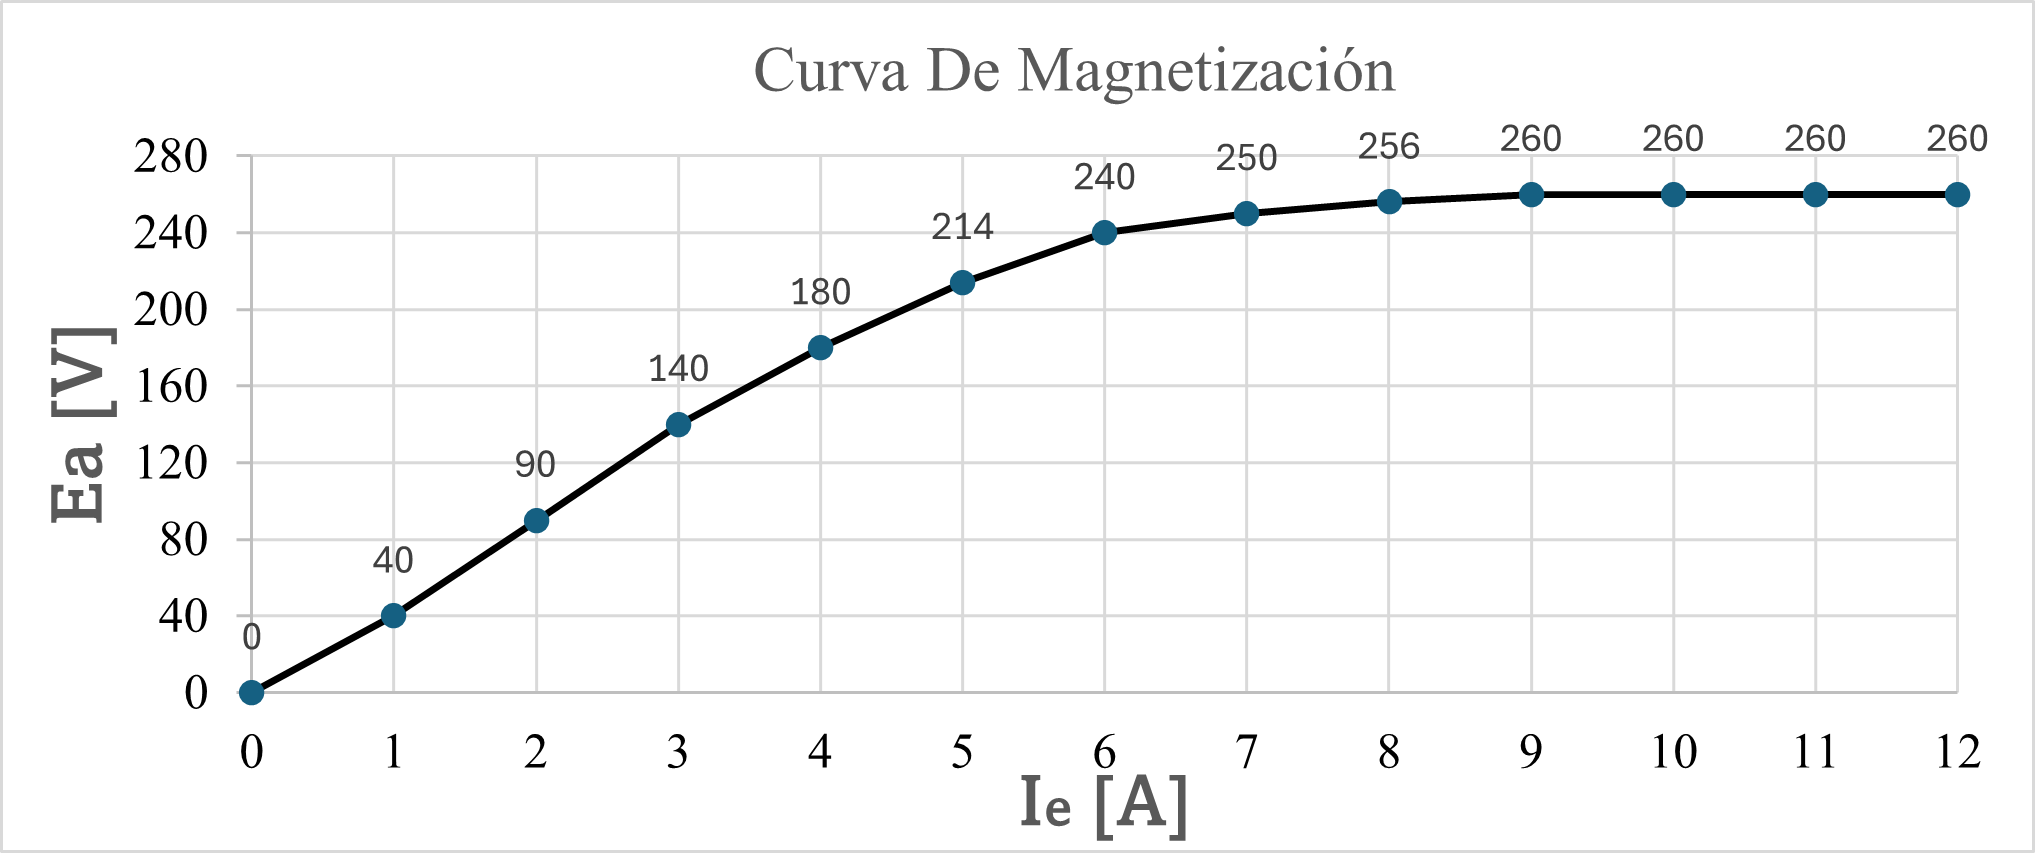
\includegraphics[width=0.8\linewidth]{img/CM_CC2.png}
    \caption{Curva de Magnetización a 1000[rpm]}
\end{figure}



Considerando esta curva, responda las siguientes preguntas. Para los cálculos puede despreciar la reacción de armadura y la caída de voltaje en las escobillas.

\begin{enumerate}[label=\alph*)]
    \item(1.5 puntos) Si el generador se conecta con excitación independiente, a tensión nominal, alimentando el circuito de campo a  $\displaystyle 60[ V]$ calcule la corriente por la armadura y potencia generada.
    \item(1.0 punto) Si la velocidad de giro aumenta a $\displaystyle 1200[ rpm]$, indique la potencia que se genera en estas condiciones y concluya respecto a la saturación de la máquina.
    \item(0.5 puntos) Considere que estando en las condiciones del inciso b) y que solo tiene acceso al circuito de campo, si se desea que la tensión de la armadura sea igual que en el inciso a) mencione y calcule la modificación que realizará al circuito de campo.
    \item(1.5 puntos) En las condiciones asignadas inicialmente ($\displaystyle 1000[ rpm]$), considere que el generador se conecta con excitación shunt (en paralelo, en derivación) a tensión nominal, calcule nuevamente la corriente por la armadura y potencia generada. Comente acerca de las ventajas y desventajas respecto a la conexión con excitación independiente.
    \item(1.5 puntos) Debido a temas de seguridad, la corriente de armadura no debe superar los $\displaystyle 200[ A]$ en estado estacionario, (ahora usted puede acceder a todo el circuito de la máquina) indique y calcule qué modificaciones debe realizar a ambos tipos de conexión, para que se cumpla esta restricción.
\end{enumerate} 
